\section{Data Preparation}

Mit den Erkenntnissen aus der vorherigen Phase beginnt nun die Aufbereitung der Daten. Jede Komponente bzw. jedes System hat im Project RA Application Conditions einen Ordner \glqq 10\char95 Project
Answers\grqq{}. Nutzt ein Projekt nun beispielsweise das Achszähler-System AzS350U und hat die Anwendungsregeln des Systems bewertet, dann müssen diese bewerteten Anwendungsregeln in ein neues Modul 
in dem \glqq 10\char95 Project Answers\grqq{} Ordner des Achszähler-Systems geschrieben werden. Mit den Modulen, die die bewerteten Anwendungsregeln der einzelnen Komponenten und Systeme beinhalten,
kann dann das KI-System angelernt werden. 

Um das zu erreichen, müssen zunächst die 115 Module genauer untersucht werden. Dabei muss geprüft werden, ob diese Module die Anwendungsregeln so bewertet haben, wie es das Process Manual vorgibt.
Dafür muss die Iteration aus \ref*{lst:searchInLinks} erweitert werden. Es muss zusätzlich geprüft werden, ob das Modul die Attribute REQ Status bzw. REQ Progress besitzt und ob diese auch 
ausgefüllt sind. 

\begin{lstlisting}[caption={Suche nach bewerteten Anwendungsregeln},captionpos=b, label = lst:searchARSolutions]                                                       
if(hasAttribute("REQ Status", mod) 
&& hasAttribute("REQ Statement", mod)){  
    szProgress = o."REQ Status""";
    szStatement = o."REQ Statement";
    if(length(szProgress)>1 && length(szStatement)>1){ 
        put(slResults, fullName mCheck, fullName mCheck)
    }
}else if (hasAttribute("REQ Progress", mod) 
&& hasAttribute("REQ Statement", mod)){
    szProgress = o."REQ Progress""";
    szStatement = o."REQ Statement";
    if(length(szProgress)>1 && length(szStatement)>1){ 
        put(slResults, fullName mCheck, fullName mCheck)
        // ...
\end{lstlisting}

Übrig bleiben danach 41 Module aus 34 Projekten, welche nicht nur die Anwendungsregeln importiert, sondern auch nach den Vorgaben des Process Manuals bewertet haben. Als Zwischenschritt wurde daraufhin
für jedes Projekt ein Modul in meiner Sandbox erstellt. In diesem Modul wurden dann alle bewerteten Anwendungsregeln reingeschrieben. Dabei musste darauf geachtet werden, dass auschließlich die
Anwendungsregeln in das Modul geschrieben wurden und keine Überschriften oder Ähnliches. Zudem durften nur die relevanten Attribute in dem neuen Modul stehen. Alle weiteren Attribute dürfen nicht
hinzugefügt werden, da diese für das Bewerten von Anwendungsregeln irrelevant sind und die Module und somit den schlussendlichen Datensatz, welcher zum Trainieren des KI-Systems verwendet werden soll,
unnötig groß machen würden. Zudem muss, wie in Kapitel \ref*{chap:DataUnderstanding} beschrieben, überprüft werden, ob sich die Anwendungsregel unter dem Punkt 
\glqq Old Version Objects, to be reviewed and deleted: \grqq{} befindet. Dafür muss über alle Väter eines Objekts iteriert werden und geprüft werden, ob die Überschrift eines Objekts 
\glqq Old Version Objects, to be reviewed and deleted: \grqq{} ist. Der Quellcode \ref*{lst:checkOld} zeigt eine Möglichkeit, bei der eine Boolean-Variable auf true gesetzt wird, falls ein Objekt
veraltet ist. Diese Objekte werden dann nicht in das neue Modul geschrieben.

\begin{lstlisting}[caption={Prüfen, ob Objekt veraltet ist}, captionpos=b, label = lst:checkOld] 
for obj in entire mod do{ 
    oParent = parent(obj)
    bOldVersion = false;
    while (oParent != null){
        if (oParent."Object Heading""" ==  "Old Version Objects, to be reviewed and deleted:"){
            bOldVersion = true;
        }
        oParent = parent(oParent)
    }
\end{lstlisting}

Abbildung \ref*{fig:SolutionsModul} zeigt, wie ein Modul für ein Projekt dann aussieht. Erkennbar ist, dass dort lediglich die relevanten Attribute gespeichert werden. Zudem wird ein Out-Link auf die
Anwendungsregel unter RA Application Conditions gesetzt, damit nachverfolgt werden kann, von wo die Anwendungsregel ursprünglich stammt. Des Weiteren besteht der Name des Moduls aus dem Namen
des Projekt sowie der Endung \glqq \char95 Solutions\grqq{}. Dadurch wird sichergestellt, dass die Information darüber, von welchem Projekt die bewertete Anwendungsregel stammt, erhalten bleibt.

\begin{figure}[H]
    \centering
    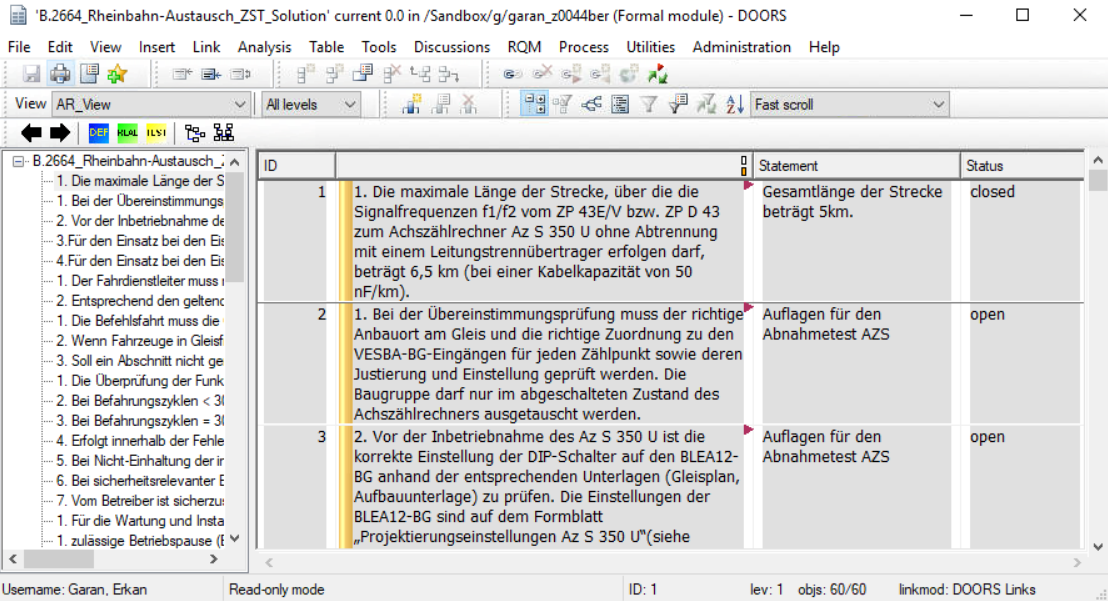
\includegraphics[width = \textwidth]{abbildungen/Solutions.PNG}
    \caption{Modul eines Projekts}
    \label{fig:SolutionsModul}
\end{figure}



% TODO

- Zwischenschritt: für jedes Projekt ein Modul in Sandbox
- dabei darauf achten, dass nur relevante Attribute kopiert werden und keine old versions
- diese dann aufteilen, auf einzelne Komponenten/Systeme durch Links
- die neuen Module dann in Projects Answers einfügen
- FERTIG